\section{Evaluation}\label{sec:eval}
The performance of our fully optimized kernels is shown in \figref{eval}. The
performance of the \ttt{big\_blocked} and \ttt{3\_level\_blocking} kernel are
consistent for all sizes of matrices but generally perform worse than the
\ttt{padded\_blocked} kernel. This indicates that the compiler's ability to
efficiently compile loops with a fixed number of iterations has a large impact
on the efficiency of the code.

Moreover, the \ttt{padded\_if} kernel expectedly performs more consistently
than the \ttt{padded\_blocked} kernel because it does not perform any
superfluous computations. Similarly the \ttt{padded\_blocked} kernel
outperforms the \ttt{padded\_if} kernel when the matrix size is a multiple of
the block size. This is because the \ttt{padded\_blocked} kernel does not pay
the overhead of dynamically selecting between two different loops.

\begin{figure}[h]
  \centering
  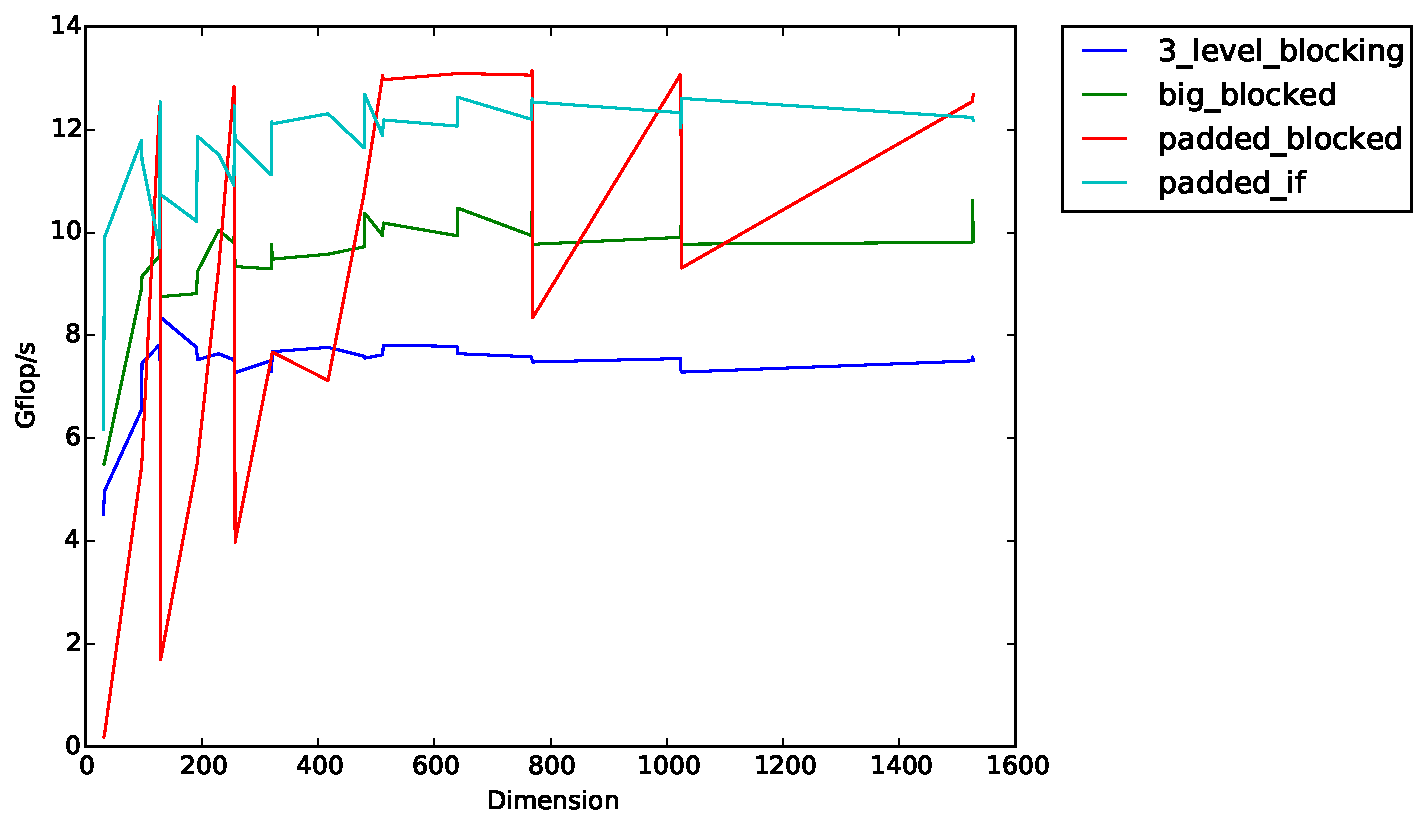
\includegraphics[width=\textwidth]{img/timing_eval.pdf}
  \caption{Evaluation of optimized kernels.}
  \label{fig:eval}
\end{figure}

The performance of our optimized kernels compared to the performance of all the
kernels is shown in \figref{eval-all}. The same plot without the \ttt{mkl} or
\ttt{blas} kernels is shown in \figref{eval-all-but-beast}. The peak Gflop/s of
our kernels is roughly 4 times lower than that of \ttt{mkl} and \ttt{blas}. On
the other hand, our kernels achieve almost 6 times the number of Gflop/s of the
naive matrix multiplication kernel.

Moreover, the running time of all kernels when run on a variety of matrices is
shown in \tabref{eval}. Notably, the \ttt{padded\_blocked} and \ttt{padded\_if}
kernels are only a couple of seconds slower than the \ttt{mkl} and \ttt{blas}
kernels.

\begin{table}[h]
  \centering
  \begin{tabular}{|c|c|}
    \hline
    \ttt{blas}               & 0:45 \\\hline
    \ttt{mkl}                & 0:45 \\\hline
    \ttt{padded\_blocked}    & 0:47 \\\hline
    \ttt{padded\_if}         & 0:48 \\\hline
    \ttt{big\_blocked}       & 0:54 \\\hline
    \ttt{3\_level\_blocking} & 0:56 \\\hline
    \ttt{annotated}          & 1:06 \\\hline
    \ttt{copyopt}            & 1:07 \\\hline
    \ttt{f2c}                & 1:11 \\\hline
    \ttt{blocked}            & 1:39 \\\hline
    \ttt{compiler}           & 1:58 \\\hline
    \ttt{basic}              & 2:04 \\\hline
  \end{tabular}
  \caption{Running time of all kernels.}
  \label{tab:eval}
\end{table}

\begin{figure}[h]
  \centering
  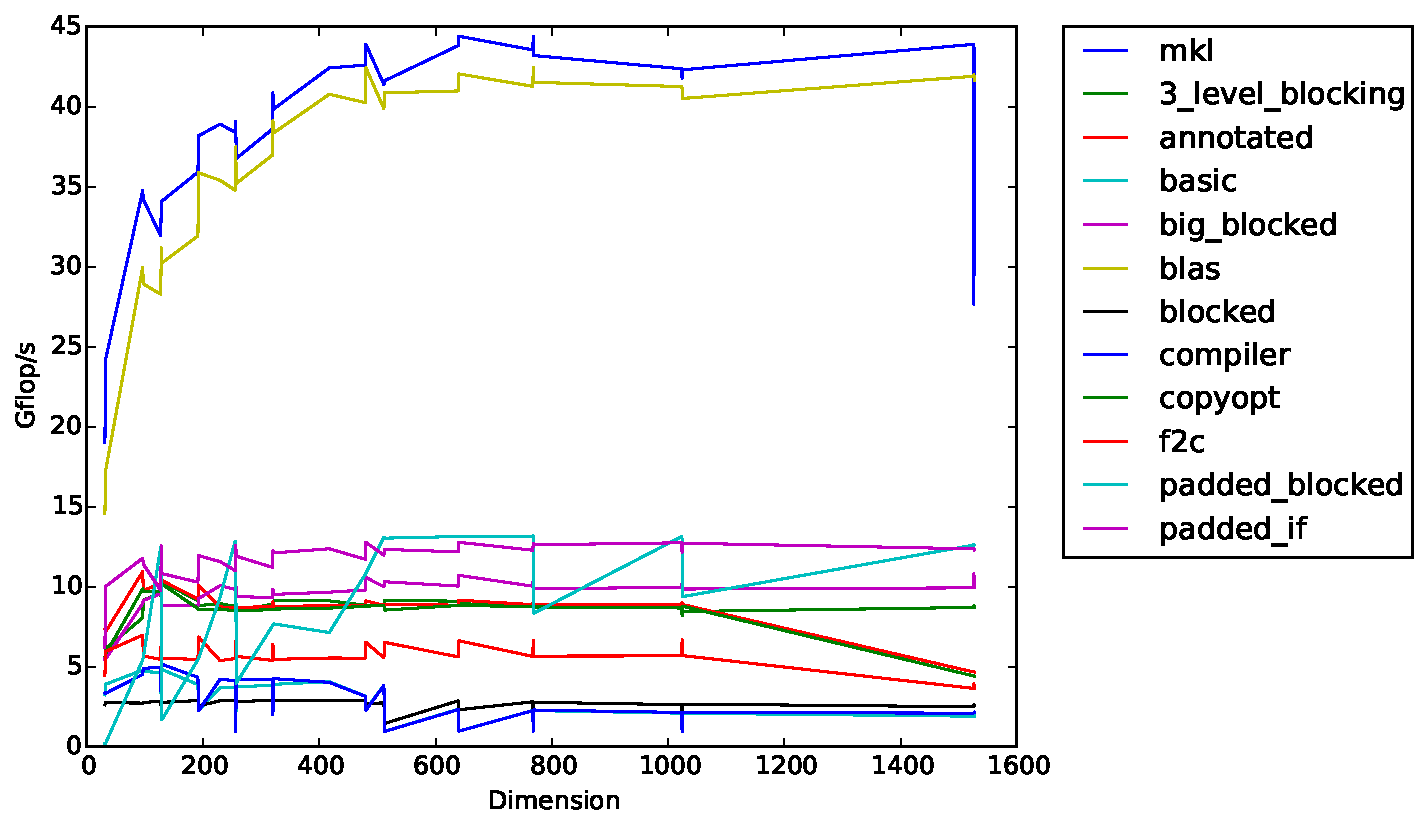
\includegraphics[width=\textwidth]{img/timing_all.pdf}
  \caption{Evaluation of all kernels.}
  \label{fig:eval-all}
\end{figure}

\begin{figure}[h]
  \centering
  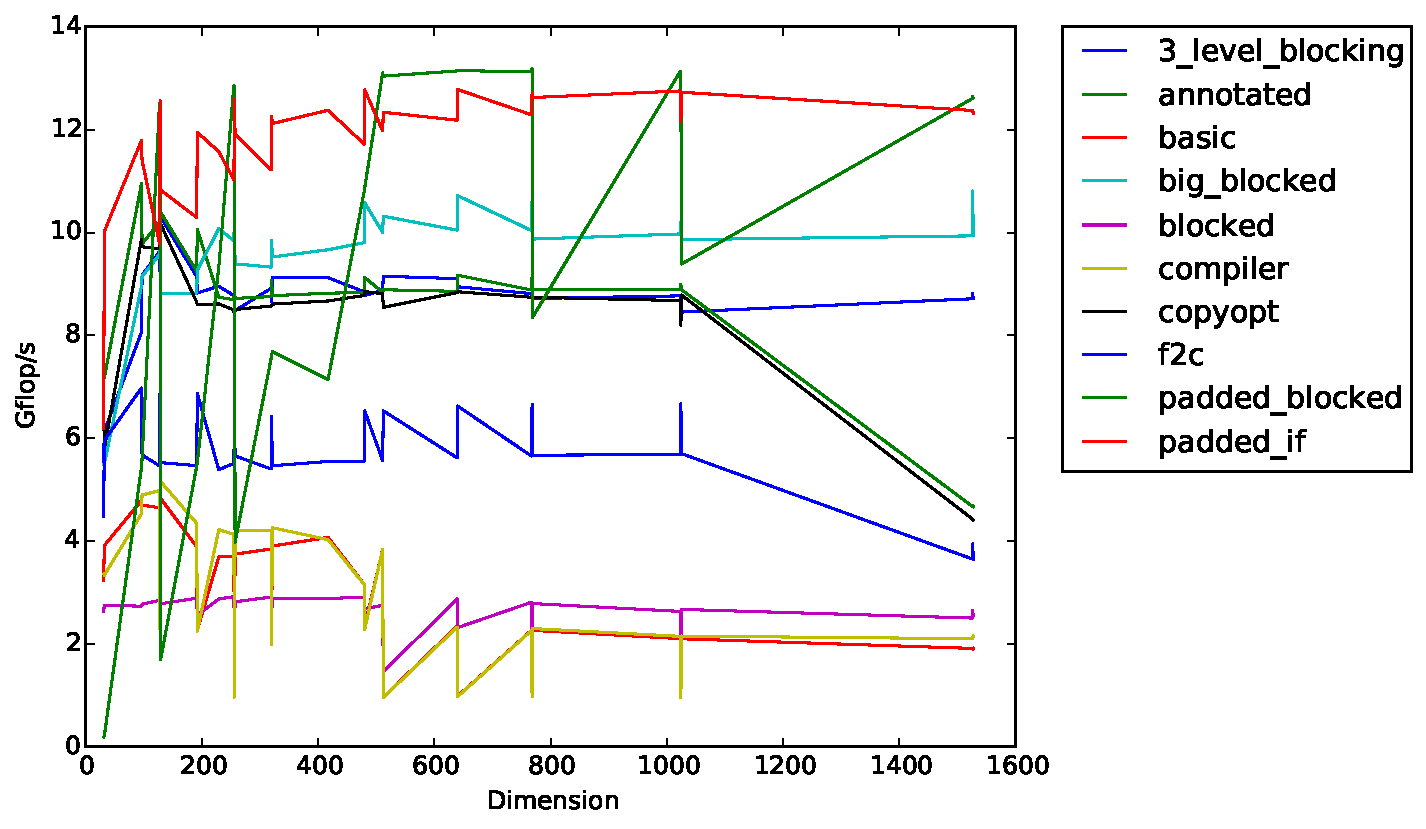
\includegraphics[width=\textwidth]{img/timing_all_but_beast.pdf}
  \caption{Evaluation of all kernels except \ttt{blas} or \ttt{mkl}.}
  \label{fig:eval-all-but-beast}
\end{figure}
